\documentclass[12pt,a4paper]{article}

\usepackage{amssymb}
\usepackage{url}
\usepackage{mathptmx}
\usepackage{float}
\usepackage{makeidx}
\usepackage{balance}
\makeindex

\usepackage{tikz}
\usetikzlibrary{positioning,arrows,calc}
\tikzset{>=stealth}

\textwidth=155mm
\textheight=240mm
\topmargin=0pt
\headheight=0pt
\oddsidemargin=-5mm
\evensidemargin=5mm
\headsep=0pt
\parindent=0pt
\renewcommand{\baselinestretch}{1.1}
\setlength{\parskip}{0.3\baselineskip plus 1pt minus 1pt}
\addtolength{\jot}{3pt}

\newtheorem{theorem}{Theorem}
\newtheorem{definition}[theorem]{Definition}
\newtheorem{axiom}[theorem]{Axiom}
\newcommand*{\ih}{\stackrel{\bullet}{=}}
\newcommand*{\qed}{\hfill\rule[-2pt]{4pt}{10pt}}
\newcommand*{\imp}{\mathbin{\rightarrow}}
\newcommand*{\comma}{,\:}
\newcommand*{\ind}{\hspace*{2em}}
\newenvironment{example}{\textbf{Example}}{}
\newenvironment{proof}{\textbf{Proof}}{\qed}

\begin{document}

\thispagestyle{empty}

\begin{center}
\textbf{\Large A Short Introduction to Set Theory}

\bigskip

\textbf{\Large Moti Ben-Ari}

\bigskip

\url{http://www.weizmann.ac.il/sci-tea/benari/}

\end{center}

\begin{small}
This is an Author Accepted Manuscript version of the following work:
Mordechai Ben-Ari, Mathematical Logic for Computer Science (Third Edition),
2012, Springer, reproduced with permission of Springer-Verlag London.
The final authenticated version is available online at:\\
http://dx.doi.org/10.1007/978-1-4471-4129-7.
\end{small}
\bigskip

\tableofcontents

\newpage

This document is based upon Appendix~A of [1] and used by permission of Springer.

The presentation of mathematical logic in [1] is based upon an informal use of set theory whose definitions and theorems are summarized here. For an elementary, but detailed, development of set theory, see [4].

I would like to express my thanks to J\o{}rgen Villadsen for his helpful suggestions.	

\section{Finite and infinite sets}

The concept of an \emph{element} is undefined, but informally the
concept is clear: an element is any identifiable object like a number,
color or node of a graph. Sets are built from elements.

\begin{definition}
A \emph{set}\index{Set} is composed of
\emph{elements}.\index{Element} $a\in S$\index{a01@$\in$} denotes
that $a$ is an element of set $S$ and $a\not\in S$\index{a02@$\not\in$} denotes that $a$ is \emph{not} an element of $S$. $\emptyset$\index{a03@$\emptyset$},  the \emph{empty set},\index{Empty set} is the set with no
elements. Capital letters like $S$, $T$ and $U$
are used for sets. The elements of sets are written within braces $\{\;\}$\index{a03a@$\{\cdots\}$}.
\end{definition}

There are two ways to define a set: (a) We can explicitly write the
elements comprising the set. If a set is large and if it is clearly
understood what its elements are, an ellipsis `$\ldots$' is used to
indicate the elements that are not listed. (b) A set may be defined by
set comprehension, where the set is specified to be composed of
all elements that satisfy a condition. 


\begin{example}\mbox{}
\begin{itemize}
\item The set of colors of a traffic light is $\{\textit{red}, \textit{yellow}, \textit{green}\}$.

\item The set of atomic elements is $\{\textit{hydrogen}, \textit{helium}, \textit{lithium}, \ldots\}$.

\item $\mathbb{Z}$,\index{a04@$\mathbb{Z}$} the set of
\emph{integers},\index{Integers} is $\{\ldots,-2,-1,0,1,2,\ldots\}$.

\item $\mathbb{N}$\index{Natural numbers}\index{a05@$\mathbb{N}$}, the set of \emph{natural numbers}, is $\{0,1,2,\ldots\}$. $\mathbb{N}$ can also be defined by \emph{set comprehension}\index{Set comprehension}\index{a05a@$\{\cdots\mid\cdots \;\}$}: $\mathbb{N}=\{n\in \mathbb{Z} \mid n\geq 0\}$. Read this as ``$\mathbb{N}$ is the set of all integers $n$ such that $n$ is greater than or equal to zero.''

\item $\mathbb{R}$\index{Real numbers}\index{a06@$\mathbb{R}$}, the set of \emph{real numbers}, can be informally defined as all numbers that can be expressed in decimal notation: $3.14159$ or $0.31459\times 10^1$.

\item $E$, the set of even natural numbers, is $\{n\in \mathbb{N} \mid n \bmod 2 = 0\}$.

\item $P$, the set of prime numbers, is:
\[
\{n\in \mathbb{N} \mid n\geq 2 \textrm{\ and for all\ } m \:(n \bmod m = 0 \textrm{\ implies\ } (m=1 \mathrm{\ or\ } m=n))\}.
\]
\end{itemize}
\end{example}

There is no meaning to the order of the elements in a set nor to
repetition of elements: $\{3,2,1,1,2,3\}=\{1,2,3\}=\{3,1,2\}$.
A set containing a single element (a \emph{singleton set}\index{Singleton})
and the element itself are not the same: $5\in \{5\}$.

\section{Subset}

\begin{definition}
Let $S$ and $T$ be sets. $S$ is a \emph{subset}\index{Subset} of
$T$, denoted $S\subseteq T$,\index{a07@$\subseteq$} iff every element of
$S$ is an element of $T$, that is, $x\in S$ implies $x \in T$. $S$ is a
\emph{proper subset}\index{Proper} of $T$, denoted $S\subset
T$\index{a08@$\subset$}, iff $S\subseteq T$ and $S\neq T$.
\end{definition}

\begin{example}
$\mathbb{N}\subset \mathbb{Z}\comma\; E \subset \mathbb{N}\comma\; \{\mathit{red},\mathit{green}\}\subset \{\mathit{red}, \mathit{yellow}, \mathit{green}\}\comma\; \{\mathit{red},\mathit{green}\}\subseteq \{\mathit{green}, \mathit{red}\}$.
\end{example}

\begin{theorem} $\emptyset \subseteq T$.
\end{theorem}
\begin{proof}
We have to show that $x \in T$ holds for all $x\in \emptyset$. But there are no elements in $\emptyset$, so the statement is vacuously true.
\end{proof}

The relationships among sets can be shown graphically by the use
of \emph{Venn diagrams}.\index{Venn diagram} These are closed curves
drawn in the plane and labeled with the name of a set. A point is in the
set iff it is within the interior of the curve. In the following diagram, $S$ is a subset of $T$ since every point within $S$ is also within $T$.

\begin{center}
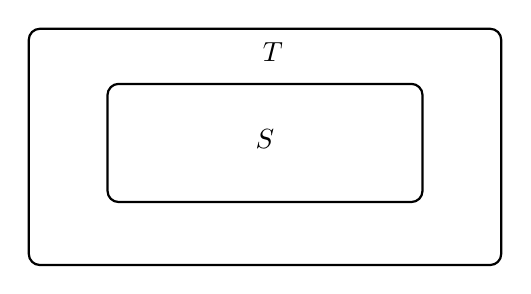
\begin{tikzpicture}
\draw[thick,rounded corners] (0,0) node[xshift=3.1cm,yshift=2.7cm] {$T$}
  rectangle +(6,3);
\draw[thick,rounded corners] (1,.8) node[xshift=2cm,yshift=.8cm] {$S$}
  rectangle +(4,1.5);
\end{tikzpicture}
\end{center}

\begin{theorem}The subset property is transitive:

\begin{enumerate}
\item If $S\subseteq T$ and $T\subseteq U$ then $S\subseteq U$.
\item If $S\subset T$ and $T\subseteq U$ then $S\subset U$.
\item If $S\subseteq T$ and $T\subset U$ then $S\subset U$.
\item If $S\subset T$ and $T\subset U$ then $S\subset U$.
\end{enumerate}
\end{theorem}

\begin{proof}
Let us prove (2). By the assumption $S\subset T$: if $x\in S$ then $x\in T$. By the assumption $T\subseteq U$ if $x\in T$ then $x\in U$. Therefore, $S\subseteq U$. We have to show that $S\neq U$. By assumption, $S \subset T$ so $S\neq T$ and there is an element $x\in T$ and $x\not \in S$. Since $T\subseteq U$, $x\in U$ and by assumption $x\not \in S$, so $S\neq U$.
\end{proof}

\section{Proving inclusion and equality of sets}

To prove $S\subseteq T$ choose an \emph{arbitrary} element $x\in S$
and show $x\in T$.

\begin{example}
Prove that every prime number greater than $2$ is odd. Formally:
\begin{eqnarray*}
S&=&\{n \in \mathbb{N} \mid n>2 \textrm{\ and \ } n\in P\}\\ 
T&=& \{n\in \mathbb{N} \mid n=2k+1 \textrm{\ for some \ } k\in \mathbb{N}\}\\
S&\stackrel{?}{\subseteq}& T\,.
\end{eqnarray*}
Let $n$ be an \emph{arbitrary} element of $S$. Suppose that $n\not\in T$. Then $n=2k$ for some $k\in \mathbb{N}$. If $k=0$ or $k=1$ so that $n=1$ or $n=2$, then $n\not>2$ and $n\not\in S$. Otherwise, $n>2$ has (at least) the factors $2,k$ that are different from $1$ and $n$, so $n\not \in S$. Since $n$ was an arbitrary element of $S$, $S\subseteq T$.
\end{example}

To prove that two sets are equal, use the following theorem whose proof is left to the reader:
\begin{theorem}\label{thm.setsequal}
\ind $S=T$ iff $S\subseteq T$ and $T\subseteq S$.
\end{theorem}

\begin{example}
Prove that $E$, the set of even natural numbers, is equal to the set of natural numbers of the form $2k$ for $k\in\mathbb{N}$. Formally:
\begin{eqnarray*}
S&=&\{n\in \mathbb{N} \mid  n \bmod 2 = 0\}\\
T&=&\{n\in \mathbb{N} \mid \textrm{\ for some\ } k\in \mathbb{N}, n=2k\}\\
S&\stackrel{?}{=}&T\,.
\end{eqnarray*}

Let $m\in S$. Then $m\bmod 2 = 0$, which by definition means there is a $k\in \mathbb{N}$ such that $m=2k+0=2k$. Therefore, $m\in T$ and $S\subseteq T$. If $m\in T$, then there is a $k$ such that $m=2k=2k+0$ so $m\bmod 2=0$. Therefore, $T\subseteq S$. By Theorem~\ref{thm.setsequal} $S=T$.
\end{example}

\section{Union, intersection and difference}


\begin{definition}\mbox{}
\begin{enumerate}
\item $S\cup T=\{x\mid x\in S \emph{\ or \ } x\in T\}$,\index{a09@$\cup$} the \emph{union}\index{Union} of $S$ and $T$, is the set consisting of those elements which are elements of \emph{either} $S$ \emph{or} $T$ or both.

\item $S\cap T=\{x\mid x\in S \emph{\ and \ } x\in T\}$,\index{a10@$\cap$} the \emph{intersection}\index{Intersection} of $S$ and $T$, is the set consisting of those elements which are elements of \emph{both} $S$ \emph{and} $T$. If $S\cap T=\emptyset$ then $S$ and $T$ are \emph{disjoint}.\index{Disjoint}

\item $S-T=\{x\mid x\in S \emph{\ and \ } x\not\in T\}$,\index{a11@$-$} the \emph{difference}\index{Difference} of $S$ and $T$, is the set of elements of $S$ that are not elements of $T$.

\item Let $U$ be understood as a universal set; then $\overline{T}$\index{a12@$\overline{T}$}, the
\emph{complement}\index{Complement} of $T$, is $U-T$.
\end{enumerate}
\end{definition}

The following Venn diagram illustrates these concepts.

\begin{center}
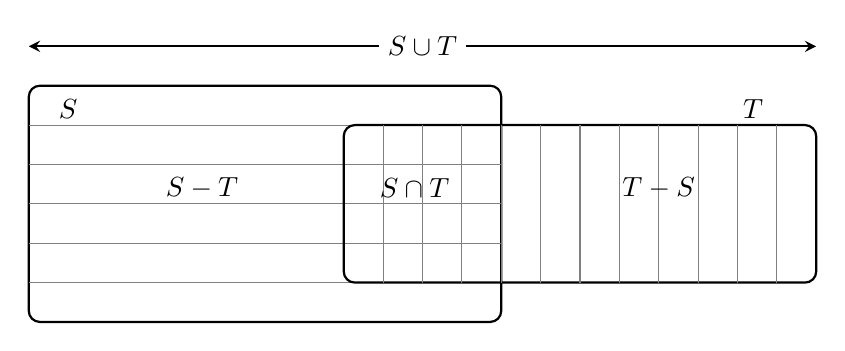
\begin{tikzpicture}
\draw[thick,rounded corners] (0,0) rectangle +(6,3);
\foreach \y in {.5,1,1.5,2,2.5}
  \draw[thin,white!50!black] (0,\y) -- (6,\y);
\draw[thick,rounded corners] (4,.5) rectangle +(6,2);
\foreach \x in {4.5,5,5.5,6,6.5,7,7.5,8,8.5,9,9.5}
  \draw[thin,white!50!black] (\x,.5) -- (\x,2.5);
\node at (.5,2.7) {$S$};
\node at (9.2,2.7) {$T$};
\node at (2.2,1.7) {$S-T$};
\node at (8,1.7) {$T-S$};
\node at (4.9,1.7) {$S\cap T$};
\draw[thick,<->] (0,3.5) -- node[fill=white] {$S\cup T$} (10,3.5);
\end{tikzpicture}
\end{center}

\begin{example} Here are some examples of the operations on sets:
\begin{displaymath}
\begin{array}{lll}
\{\mathit{red}, \mathit{yellow}\} \cup \{\mathit{red}, \mathit{green}\} &=& \{\mathit{red}, \mathit{yellow}, \mathit{green}\}, \\
\{\mathit{red}, \mathit{yellow}\} \cap \{\mathit{red}, \mathit{green}\} &=& \{\mathit{red}\}, \\
\{\mathit{red}, \mathit{yellow}\} - \{\mathit{red}, \mathit{green}\} &=& \{\mathit{yellow}\}, \\
P \cap E &=& \{2\}.
\end{array}
\end{displaymath}
\end{example}
The following theorem states some properties of the set
operators.
\begin{theorem}\label{thm.seteq}\mbox{}
\begin{enumerate}
\item $T = (T-S) \cup (S\cap T)$.

\item If $S\subseteq T$ then:
$\;\;S \cap T = S\comma \;\; S \cup T = T\comma\;\; S - T = \emptyset$.

\item If $S$ and $T$ are disjoint then $S-T=S$.

\item $S \cup \emptyset = S\comma\;\; S \cap \emptyset = \emptyset\comma\;\;
S - \emptyset = S$.
\end{enumerate}
\end{theorem}

\begin{proof}
\begin{enumerate}
\item See the Venn diagram above.

\item See the following Venn diagram.

\begin{center}
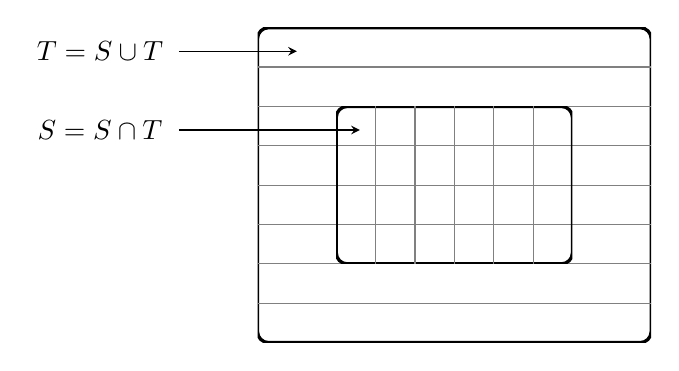
\begin{tikzpicture}
\begin{scope}
\clip (0,0) rectangle +(5,4);
\draw[very thick,rounded corners] (0,0) rectangle +(5,4);
\foreach \y in {.5,1,1.5,2,2.5,3,3.5}
  \draw[thin,white!50!black] (0,\y) -- (5,\y);
\end{scope}
\begin{scope}
\clip (1,1) rectangle +(3,2);
\draw[very thick,rounded corners] (1,1) rectangle +(3,2);
\foreach \x in {1.5,2,2.5,3,3.5}
  \draw[thin,white!50!black] (\x,0) -- (\x,4);
\end{scope}
\node at (-2,2.7) {$S=S\cap T$};
\draw[->] (-1,2.7) -- +(2.3,0);
\node at (-2,3.7) {$T=S\cup T$};
\draw[->] (-1,3.7) -- +(1.5,0);
\end{tikzpicture}
\end{center}

For example, $P \cap \mathbb{N} = P,\; P \cup \mathbb{N} = \mathbb{N}$.

\item $S-T=\{x\mid x\in S \textrm{\ and \ } x\not\in T\}$. By definition, $S$ and $T$ are disjoint means $S\cap T=\emptyset$, that is, $x\in S$ implies $x\not \in T$, so every element in $S-T$ is in $S$.  

\item Let us prove $S\cap \emptyset = \emptyset$. $S\cap \emptyset=\{x\mid x\in S \textrm{\ and \ } x\in \emptyset\}$, but there are no $x$ such that $x\in \emptyset$ so there are no elements in $S\cap \emptyset$.
\end{enumerate}\vspace{-4ex}
\end{proof}

The operators $\cup$ and $\cap$ are commutative, associative and distributive.

\begin{theorem}\mbox{}
\begin{enumerate}
\item $S \cup T = T \cup S$.
\item $S \cap T = T \cap S$.
\item $(S \cup T) \cup U = S \cup (T\cup U)$.
\item $(S \cap T) \cap U = S \cap (T\cap U)$.
\item $S \cup (T\cap U) = (S \cup T) \cap (S \cup U)$.
\item $S \cap (T\cup U) = (S \cap T) \cup (S \cap U).$
\end{enumerate}
\end{theorem}
The reader is invited to give informal proofs of these properties by drawing Venn diagrams.


\section{Sequences}
\index{Sequence}

\begin{definition}\label{def.sequences}
Let $S$ be a set. A \emph{finite sequence of elements of $S$} is a function:\footnote{\emph{Functions} and the symbol $\mapsto$ are formally defined in Section~\ref{s.function}.}
\[
f:\{0,\ldots,n-1\}\mapsto S\,.
\]
The \emph{length} of the sequence is $n$. An \emph{infinite sequence of elements of $S$} is a function:
\[
f:\mathbb{N}\mapsto S\,.
\]
\end{definition}

\begin{example}
Let $S$ be the set of three colors $\{\mathit{red},
\mathit{yellow}, \mathit{green}\}$. Suppose that you at are a traffic light and see a green light, but before you can cross the street, the light changes and you have to wait until the light is green again. $L_1$, the finite sequence of colors that you will see until you cross, is:
\begin{displaymath}
f_{L_1}(0)=\mathit{green},\; f(1)_{L_1}=\mathit{yellow},\; f(2)_{L_1}=\mathit{red},\; f(3)_{L_1}=\mathit{green}\,.
\end{displaymath}
$L_2$, the infinite sequence of colors that the light shows (assuming that it is always on), is:
\begin{displaymath}
f_{L_2}(0)=\mathit{green},\; f_{L_2}(1)=\mathit{yellow},\; f_{L_2}(2)=\mathit{red},\; f_{L_2}(3)=\mathit{green},\; f_{L_2}(4)=\mathit{yellow},\; \ldots,
\end{displaymath}
where the ellipsis $\ldots$ indicates that we know how to continue
constructing the sequence. Alternatively, we could formally define the infinite
sequence $L_2$ as:
\begin{displaymath}
\begin{array}{ll}
f_{L_2}(i)=\mathit{green}&\mathrm{if}\; i\bmod 3 = 0\\
f_{L_2}(i)=\mathit{yellow}&\mathrm{if}\; i\bmod 3 = 1\\
f_{L_2}(i)=\mathit{red}&\mathrm{if}\; i\bmod 3 = 2\,.
\end{array}
\end{displaymath}
\end{example}
The elements of a sequence are listed within parentheses $(\,)$\index{a12a@$(\cdots)$} to differentiate them from the elements of sets which are written within braces $\{\,\}$. In a sequence $(s_0, s_1, s_2, \ldots)$, $s_i=f(i)$:

\[
L_2=(\mathit{green},\; \mathit{yellow},\; \mathit{red},\; \mathit{green},\; \mathit{yellow},\; \mathit{red},\; \ldots)\,.
\]
\begin{definition}
A finite sequence of length $n$ is called an \emph{n-tuple}. The
following terms are also used: a $2$-tuple is a \emph{pair}, a $3$-tuple
is a \emph{triple}, a $4$-tuple is a \emph{quadruple}.
\end{definition}

\begin{example} Examples of sequences:
\begin{itemize}
\item A $1$-tuple: $(\mathit{red})$.
\item A pair: $(5, 25)$.
\item A triple: $(\mathit{red}, \mathit{yellow}, \mathit{green})$.
\item A different triple: $(\mathit{red}, \mathit{green}, \mathit{yellow})$.
\item A triple with repeated elements: $(\mathit{red}, \mathit{green}, \mathit{green})$.
\item An infinite sequence: $(1, 2, 2, 3, 3, 3, 4, 4, 4, 4, \ldots)$.
\end{itemize}
\end{example}
It is important to understand that a sequence can have multiple occurrences of the same element, whereas a set has only one occurrence of each element:
\begin{eqnarray*}
(\mathit{green},\; \mathit{yellow},\; \mathit{red},\; \mathit{green})&\neq& (\mathit{green},\; \mathit{yellow},\; \mathit{red})\\
\{\mathit{green},\; \mathit{yellow},\; \mathit{red},\; \mathit{green}\}&=& \{\mathit{green},\; \mathit{yellow},\; \mathit{red}\}\,.
\end{eqnarray*}

\section{Cartesian product}
\begin{definition}
Let $S_{1}, \ldots, S_{n}$ be sets. $S_{1}\times\cdots\times S_{n}$,\index{a12b@$\times$} their \emph{Cartesian product}\index{Cartesian product}, is the set of $n$-tuples $(s_1,\ldots,s_n)$, such that $s_i\in S_{i}$. If all the sets $S_{i}$ are the same set $S$, the notation $S^{n}$ is used for $S\times\cdots\times S$.
\end{definition}
The case $n=2$  is very common. Let $S$ and $T$ be sets. $S\times T$ is the set of all pairs $(s,t)$ such that $s\in S$ and $t\in T$.

\begin{example}\mbox{}
\begin{itemize}
\item $\mathbb{R} \times \mathbb{R} = \mathbb{R}^{2}$ is the set of
all pairs of real numbers. This set can be used to represent coordinates in the plane. The term Cartesian plane or Cartesian coordinates is often used for this set.
\item $\mathbb{N} \times \{\mathit{red}, \mathit{yellow},
\mathit{green}\}$ is the set of all pairs whose first element is a
number and whose second element is a color. This set could be used to represent the
color of a traffic light at different points of time: $(28,\mathit{red})$.
\item $\mathbb{N}^3$ can be used to represent dates as (day,month,year): $(11,12,1948)$.
\item $\mathbb{N}^3$ can also be used to represent times as (hours,minutes,seconds): $(16,38,52)$. Alternatively, $\mathbb{N}\times \mathbb{N} \times \mathbb{R}$ or $\mathbb{N}^2 \times \mathbb{R}$ can represent times with fractions of a second: $(16,38,52.83)$.
\end{itemize}
\end{example}

We leave it to the reader to prove the distributive laws for Cartesian products:
\begin{theorem}\mbox{}
\begin{enumerate}
\item $S\times (T \cap U) = (S \times T) \cap (S\times U)$.
\item $S\times (T \cup U) = (S \times T) \cup (S\times U)$.
\item $(S \times T) \cap (U\times V) = (S \cap U) \times (T\cap V)$.
\item $(S \times T) \cup (U\times V) = (S \cup U) \times (T\cup V)$.
\end{enumerate}
\end{theorem}


\section{Relations}\label{s.relation}

\begin{definition}
Let $S_1, S_2, \ldots$ be sets. An \emph{$n$-ary relation} $\mathbb{R}$ is a subset of $S_{1}\times \cdots \times S_{n}$. $\mathbb{R}$ is said to be a relation \emph{on} $S_{1}\times \cdots \times S_{n}$. \index{Relation}
\end{definition}
\vspace{-2ex}
For $n=1$, a subset of $S_1$ is called a \emph{unary relation}. For $n=2$, a subset of $S_1\times S_2$ is called a \emph{binary relation}.\footnote{Velleman [3, Definition 4.2.1, p. 171] uses the term \emph{relation} for what we call a \emph{binary relation}. In mathematical logic, $n$-ary relations are used to define interpretations for $n$-ary predicates [2, Definition 7.16, p. 136], so we use the more general definition.}



\begin{example}
Here are some relations over $\mathbb{N}^k$ for various $k\ge 1$:
\begin{itemize}
\item The set of prime numbers $P$ is a relation on
$\mathbb{N}^1=\mathbb{N}$.

\item
$SQ = \{(n_1,n_2)\in \mathbb{N}^2\mid n_2=n_1^2\}$ is a relation on
$\mathbb{N}^2$; it is the set of pairs of numbers and their squares:
$(4,16)\in SQ\comma (7,49)\in SQ\comma (10,99)\not \in SQ$.

\item $RP$ is the set of relatively prime numbers, that is, pairs of natural numbers that have no common divisor except for $1$:
\[
RP = \{(n,m)\in \mathbb{N}^2\mid \textrm{\ for all\ }k\: (n \bmod k = 0 \;\textrm{and}\;m \bmod k = 0 \;\textrm{imply}\; k = 1)\}\,.
\]
Examples are:
$(4,9)\in RP\comma (15,28) \in RP\comma (14,63)\not\in RP$.

\item $PT$, Pythagorean triples, are triples of values that can be the lengths of the sides of a right triangle:
\[
\{(x,y,z) \in \mathbb{N}^3\mid x^{2}+y^{2}=z^{2}\}\,.
\]
Examples are: $(3,4,5)\in PT\comma (8,15,17)\in PT\comma (6,8,9)\not\in PT$.
 
\item Let $F$ be the set of quadruples $\{(x,y,z,n)\in \mathbb{N}^4\mid x,y,z>0, n>2 \;\textrm{and}\; x^{n}+y^{n}=z^{n}\}$. Fermat's Last Theorem (which was recently proved) states that $F=\emptyset$, the empty set.
\end{itemize}
\end{example}

\begin{definition}\label{def.reflextrans}
Let $S$ be a set and $R$ a binary relation on $S^{2}$.
\begin{enumerate}
\item $R$ is \emph{reflexive} iff $R(x,x)$ for all $x\in S$.
\item $R$ is \emph{symmetric} iff $R(x_{1},x_{2})$ implies
$R(x_{2},x_{1})$.
\item $R$ is \emph{transitive} iff $R(x_{1},x_{2})$ and $R(x_{2},x_{3})$
imply $R(x_{1},x_{3})$.
\end{enumerate}
\end{definition}

\begin{definition}
$R^{*}$\index{a13@$R^{*}$}, the \emph{reflexive transitive closure of a binary relation $\mathbb{R}\subseteq S\times S$},
\index{Reflexive transitive closure} is the smallest relation that satisfies:
\begin{enumerate}
\item $R\subseteq R^{*}$.
\item $R^{*}(x,x)$ for any $x\in S$.
\item For any $x_1,x_2,x_3\in S$, if $R^{*}(x_{1},x_{2})$ and
$R^{*}(x_{2},x_{3})$ then $R^{*}(x_{1},x_{3})$.
\end{enumerate}
\end{definition}

\begin{example}
Consider the set $G=\{a,b,c,d,e,f,g\}$ and the relation $\rho$ defined by:
\[
\begin{array}{llllll}
\rho(a,b)\,, & \rho(b,a)\,, & \rho(b,d)\,, & \rho(d,a)\,,& \rho(c,e)\,,\\
\rho(f,e)\,,&\rho(f,c)\,,&\rho(c,g)\,,&\rho(g,f)\,,&\rho(g,g)\,.\\
\end{array}
\]
It is easy to visualize the relation by drawing a graph with a node for each element of $G$ and a directed arrow from node $n_1$ to node $n_2$ if $\rho(n_1,n_2)$:
\begin{center}
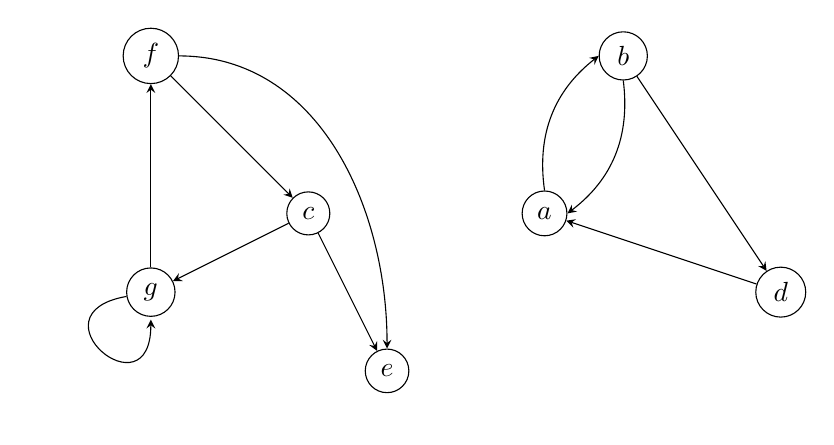
\begin{tikzpicture}
\node[draw,circle] (a) at (1,0)   {$a$};
\node[draw,circle] (b) at (2,2)   {$b$};
\node[draw,circle] (c) at (-2,0)  {$c$};
\node[draw,circle] (d) at (4,-1)  {$d$};
\node[draw,circle] (e) at (-1,-2) {$e$};
\node[draw,circle] (f) at (-4,2)  {$f$};
\node[draw,circle] (g) at (-4,-1) {$g$};
\draw[->] (g) edge[in=-90,out=190,loop] (g);

\draw[->,bend left=30] (a.north) to (b.west);
\draw[->] (b) to (d);
\draw[->] (d) to (a);
\draw[->,bend left=30] (b.south) to (a.east);

\draw[->] (f) -- (c);
\draw[->] (c) -- (e);
\draw[->] (c) -- (g);
\draw[->] (g) -- (f);
\draw[->] (f) edge[out=0,in=90] (e);
\end{tikzpicture}
\end{center}
The relation $\rho$ is not reflexive: although the relation is reflexive at node $g$ since $\rho(g,g)$ is in the relation, the relation does not include $\rho(e,e)$ and similarly for the other nodes. The relation is also not transitive: although the relation is transitive for the nodes $f,c,e$ since $\rho(f,c), \rho(c,e), \rho(f,e)$ are in the relation, the relation does not include $\rho(g,e)$ even though it does include $\rho(g,f),\rho(f,e)$.

$\rho^{*}$, the reflexive transitive closure of $\rho$, includes $\rho^{*}(n,n)$ for every $n\in G$, as well as $\rho^{*}(n_1,n_2)$ if there exists a \emph{path} $n_1,\ldots,n_2$ in the graph from $n_1$ to $n_2$.

There are no elements in $\rho$ such that $\rho(x,y)$ for $x\in \{a,b,d\}$ and $y\in\{c,e,f,g\}$, nor are there such elements in $\rho^{*}$. If you look again at (3) in the definition, we have to ensure $\rho^{*}(x_1,x_3)$ only if $R^{*}(x_{1},x_{2})$ and $R^{*}(x_{2},x_{3})$, but there are no such elements in the relation or its reflexive transitive closure, so the requirement is vacuous.
\end{example}

\section{Functions}\label{s.function}

\begin{definition}\label{def.relfunc}
A relation $F$ on $S_{1}\times \cdots \times S_{n}$ is a \emph{function} \index{Function} iff for every $n\!\!-\!\!1$-tuple $(x_{1},\ldots,x_{n-1})\in S_{1}\times \cdots \times S_{n-1}$, there is at most one $x_{n}\in S_{n}$, such that $F(x_{1},\ldots,x_{n})$.
\end{definition}

\smallskip

\begin{example}
The relation $SQ = \{(n_1,n_2),n_1,n_2\in \mathbb{Z}\mid  n_2=n_1^2\}$ is a function because for each integer, there is exactly one integer that is its square. The relation $SQRT = \{(n_1,n_2),n_1,n_2\in \mathbb{Z}\mid n_2^2=n_1\}$ is \emph{not} a function because there are integers that have two (integer) square roots, one positive and one negative, for example, $(7)^2=49$ and $(-7)^2=49$.
\end{example}

\begin{definition}
Here are some terms used with functions:
\begin{enumerate}
\item The \emph{domain}\index{Domain} of $F$ is the
set of all $(x_{1},\ldots,x_{n-1})\in S_{1}\times \cdots \times
S_{n-1}$ for which (exactly one)
\(x_{n}=F(x_{1},\ldots,x_{n-1})\) exists.

\item The \emph{range}\index{Range} of $F$ is the set
of all $x_{n}\in S_{n}$ such that
\(x_{n}=F(x_{1},\ldots,x_{n-1})\) for at least one
$(x_{1},\ldots,x_{n-1})$.

\item $F$ is \emph{total} if the domain of $F$ is
all of $S_{1}\times \cdots \times S_{n-1}$; otherwise, $F$
is \emph{partial}.\index{Total}\index{Partial}

\item $F$ is \emph{injective} or \emph{one-to-one} iff
\index{Injective}
$(x_{1},\ldots,x_{n-1}) \neq (y_{1},\ldots,y_{n-1})$ implies that
\[F(x_{1},\ldots,x_{n-1}) \neq
F(y_{1},\ldots,y_{n-1}).\]

\item $F$ is \emph{surjective} or \emph{onto} iff its range is
all of $S_{n}$.\index{Surjective}

\item $F$ is \emph{bijective} (\emph{one-to-one and onto}) iff it
is injective and surjective.\index{Bijective}
\end{enumerate}
\end{definition}

\textbf{Notation}

The notation $F:S_1\times \cdots S_{n-1}\mapsto S_n$\index{a14@$\mapsto$} is used instead of $F(x_{1},\ldots,x_{n})\in S_n$, where $(x_{1},\ldots,x_{n-1})\in S_{1}\times \cdots \times S_{n-1}$.

Similarly, the value of the function for an element of the domain can use functional notation or an expression can be given. For the example above, $n_2=SQ(n_1)=n_1^2$ for $n_1,n_2\in \mathbb{Z}$.


\begin{example}
Figure~\ref{fig.m2} shows the function:
\[
M2: \{0,1,2,3,4,5,6\} \mapsto \{0,1\}\,, \textrm{\ where \ } M2(n) = n \bmod 2\,,
\]
which is surjective (onto) but not injective (one-to-one).

Figure~\ref{fig.m2p} shows the function:
\[
M2': \{0,1,2,3,4,5,6\} \mapsto \{0,1,2,3,4,5,6\}\,, \textrm{\ where \ } M2'(n) = n \bmod 2\,,
\]
which is neither surjective nor injective:
\end{example}

\begin{figure}[H]
\begin{minipage}{.45\textwidth}
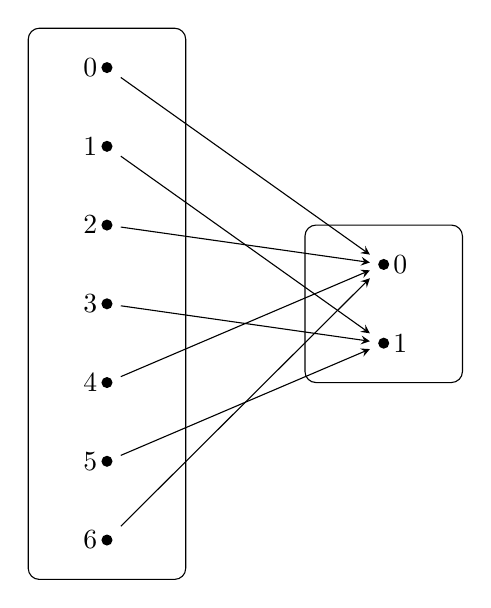
\begin{tikzpicture}
\draw[rounded corners] (0,0) rectangle +(2,7);
\fill (1,6.5) coordinate (zero) circle(2pt) node[left] {$0$};
\fill (1,5.5) coordinate (one) circle(2pt) node[left] {$1$};
\fill (1,4.5) coordinate (two) circle(2pt) node[left] {$2$};
\fill (1,3.5) coordinate (three) circle(2pt) node[left] {$3$};
\fill (1,2.5) coordinate (four) circle(2pt) node[left] {$4$};
\fill (1,1.5) coordinate (five) circle(2pt) node[left] {$5$};
\fill (1,.5) coordinate (six) circle(2pt) node[left] {$6$};

\begin{scope}[xshift=10em]
\draw[rounded corners] (0,2.5) rectangle +(2,2);
\fill (1,4) coordinate (zero-r) circle(2pt) node[right] {$0$};
\fill (1,3) coordinate (one-r)   circle(2pt) node[right] {$1$};

\foreach \y in {zero,two,four,six}
  \draw[->] ($(\y)!.05!(zero-r)$) -- ($(\y)!.95!(zero-r)$);
\foreach \y in {one,three,five}
  \draw[->] ($(\y)!.05!(one-r)$) -- ($(\y)!.95!(one-r)$);
\end{scope}
\end{tikzpicture}
\caption{Surjective but not injective}\label{fig.m2}
\end{minipage}
\hspace{3em}
\begin{minipage}{.45\textwidth}
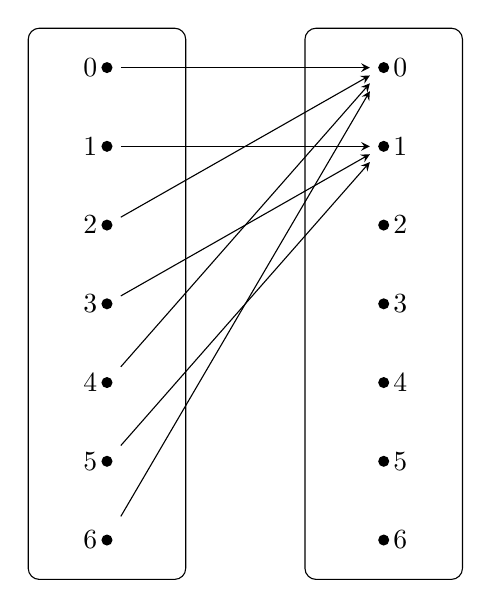
\begin{tikzpicture}
\draw[rounded corners] (0,0) rectangle +(2,7);
\fill (1,6.5) coordinate (zero) circle(2pt) node[left] {$0$};
\fill (1,5.5) coordinate (one) circle(2pt) node[left] {$1$};
\fill (1,4.5) coordinate (two) circle(2pt) node[left] {$2$};
\fill (1,3.5) coordinate (three) circle(2pt) node[left] {$3$};
\fill (1,2.5) coordinate (four) circle(2pt) node[left] {$4$};
\fill (1,1.5) coordinate (five) circle(2pt) node[left] {$5$};
\fill (1,.5) coordinate (six) circle(2pt) node[left] {$6$};

\begin{scope}[xshift=10em]
\draw[rounded corners] (0,0) rectangle +(2,7);
\fill (1,6.5) coordinate (zero-r) circle(2pt) node[right] {$0$};
\fill (1,5.5) coordinate (one-r) circle(2pt) node[right] {$1$};
\fill (1,4.5) coordinate (two-r) circle(2pt) node[right] {$2$};
\fill (1,3.5) coordinate (three-r) circle(2pt) node[right] {$3$};
\fill (1,2.5) coordinate (four-r) circle(2pt) node[right] {$4$};
\fill (1,1.5) coordinate (five-r) circle(2pt) node[right] {$5$};
\fill (1,.5) coordinate (six-r) circle(2pt) node[right] {$6$};

\foreach \y in {zero,two,four,six}
  \draw[->] ($(\y)!.05!(zero-r)$) -- ($(\y)!.95!(zero-r)$);
\foreach \y in {one,three,five}
  \draw[->] ($(\y)!.05!(one-r)$) -- ($(\y)!.95!(one-r)$);
\end{scope}
\end{tikzpicture}
\caption{Neither surjective nor injective}\label{fig.m2p}
\end{minipage}
\end{figure}

\begin{figure}[H]
\begin{minipage}{.45\textwidth}
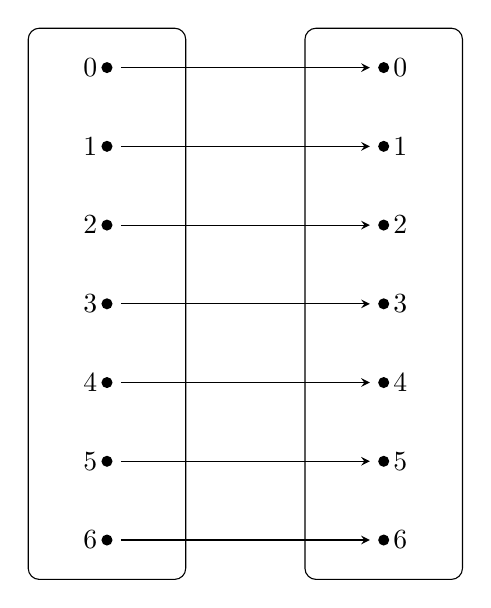
\begin{tikzpicture}
\draw[rounded corners] (0,0) rectangle +(2,7);
\fill (1,6.5) coordinate (zero) circle(2pt) node[left] {$0$};
\fill (1,5.5) coordinate (one) circle(2pt) node[left] {$1$};
\fill (1,4.5) coordinate (two) circle(2pt) node[left] {$2$};
\fill (1,3.5) coordinate (three) circle(2pt) node[left] {$3$};
\fill (1,2.5) coordinate (four) circle(2pt) node[left] {$4$};
\fill (1,1.5) coordinate (five) circle(2pt) node[left] {$5$};
\fill (1,.5) coordinate (six) circle(2pt) node[left] {$6$};

\begin{scope}[xshift=10em]
\draw[rounded corners] (0,0) rectangle +(2,7);
\fill (1,6.5) coordinate (zero-r) circle(2pt) node[right] {$0$};
\fill (1,5.5) coordinate (one-r) circle(2pt) node[right] {$1$};
\fill (1,4.5) coordinate (two-r) circle(2pt) node[right] {$2$};
\fill (1,3.5) coordinate (three-r) circle(2pt) node[right] {$3$};
\fill (1,2.5) coordinate (four-r) circle(2pt) node[right] {$4$};
\fill (1,1.5) coordinate (five-r) circle(2pt) node[right] {$5$};
\fill (1,.5) coordinate (six-r) circle(2pt) node[right] {$6$};

\foreach \y/\z in {zero/zero-r,one/one-r,two/two-r,three/three-r,four/four-r,five/five-r,six/six-r}
  \draw[->] ($(\y)!.05!(\z)$) -- ($(\y)!.95!(\z)$);
\end{scope}
\end{tikzpicture}
\caption{Surjective and injective}\label{fig.m7}
\end{minipage}
\hspace{3em}
\begin{minipage}{.45\textwidth}
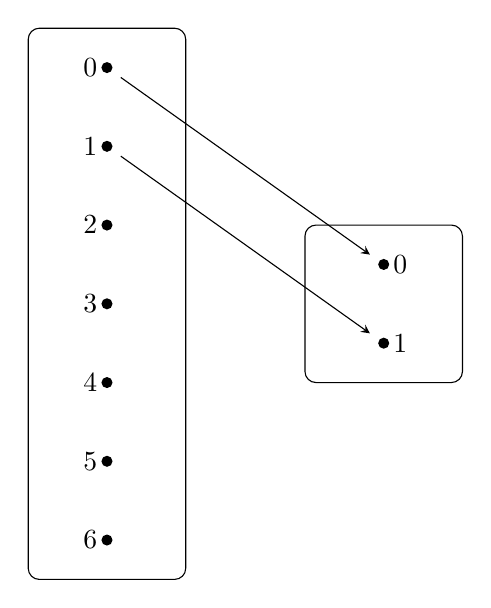
\begin{tikzpicture}
\draw[rounded corners] (0,0) rectangle +(2,7);
\fill (1,6.5) coordinate (zero) circle(2pt) node[left] {$0$};
\fill (1,5.5) coordinate (one) circle(2pt) node[left] {$1$};
\fill (1,4.5) coordinate (two) circle(2pt) node[left] {$2$};
\fill (1,3.5) coordinate (three) circle(2pt) node[left] {$3$};
\fill (1,2.5) coordinate (four) circle(2pt) node[left] {$4$};
\fill (1,1.5) coordinate (five) circle(2pt) node[left] {$5$};
\fill (1,.5) coordinate (six) circle(2pt) node[left] {$6$};

\begin{scope}[xshift=10em]
\draw[rounded corners] (0,2.5) rectangle +(2,2);
\fill (1,4) coordinate (zero-r) circle(2pt) node[right] {$0$};
\fill (1,3) coordinate (one-r)   circle(2pt) node[right] {$1$};

\foreach \y in {zero}
  \draw[->] ($(\y)!.05!(zero-r)$) -- ($(\y)!.95!(zero-r)$);
\foreach \y in {one}
  \draw[->] ($(\y)!.05!(one-r)$) -- ($(\y)!.95!(one-r)$);
\end{scope}
\end{tikzpicture}
\caption{Surjective and injective but not total}\label{fig.m2pp}
\end{minipage}
\end{figure}
Figure~\ref{fig.m7} shows the function:
\[
M7: \{0,1,2,3,4,5,6\} \mapsto \{0,1,2,3,4,5,6\}\,, \textrm{\ where \ } M7(n) = n \bmod 7\,,
\]
which is bijective, because it is both surjective (onto) and injective (one-to-one).

Figure~\ref{fig.m2pp} shows the function:
\[
M2'': \{0,1,2,3,4,5,6\} \mapsto \{0,1\}\,, \textrm{\ where \ } M2''(n) = n \bmod 2\,,
\]
which is bijective, but it is a partial function because the domain is not all of $\{0,1,2,3,4,5,6\}$.


\begin{example}
$SQ= \{(n_1,n_2),n_1,n_2\in\mathbb{Z}\mid n_2=n_1^2\}$ is a total function. Its domain is all of $\mathbb{Z}$, but its range is
only the subset of $\mathbb{Z}$ consisting of all squares. Therefore
$SQ$ is not surjective and thus not bijective. It is also not injective because it is possible that $n_1 \neq n_2$, but $n_1^2=n_2^2$, for example, $7\neq -7$ but $49=49$.
\end{example}

\begin{example}
Let $\{a_0,\ldots,a_{n-1}\} \in \mathbb{N}$ and define the set:
\[
CY_{\{a_0,\ldots,a_{n-1}\}} =\{(a_k,a_{k+1},\ldots,a_{(k+n-1)\bmod n}) \mid  k\in \{0,\ldots,n-1\}\}\,.\footnote{For $k=n-1$, we need to compute $(k+n-1) \bmod n =(2n-2) \bmod n$. But adding a multiple of $n$ does not change the modulus, so $(2n-2) \bmod n = (2n-2+(-n)) \bmod n = (n-2) \bmod n = n-2$ as expected. When $n=5$ as in the example, $(k+n-1)\bmod 5=(5-1+5-1)\bmod 5= (10-2+(-5))\bmod 5 = 3\bmod 5 = 3$, and the last element of $CY$ is $(a_4,a_0,a_1,a_2,a_3)$.}
\]
Each $CY$ is a set of sequences whose elements are cyclic. For example:
\begin{eqnarray*}
CY_{\{2,16,11,14,82\}}&=&\{(2,16,11,14,82),\;(16,11,14,82,2),\\
&&(11,14,82,2,16),\;(14,82,2,16,11),\;(82,2,16,11,14)\}\,.
\end{eqnarray*}
We can define function for shifting left and right:
\begin{eqnarray*}
\textrm{left\_shift}(a_0,a_1,\ldots,a_{n-2},a_{n-1})&=&(a_1,\ldots,a_{n-2},a_{n-1},a_0)\\
\textrm{right\_shift}(a_0,a_1,\ldots,a_{n-2},a_{n-1})&=&(a_{n-1},a_0,a_1,\ldots,a_{n-2})\,.
\end{eqnarray*}
Clearly, the domain and the range of these functions is all of $CY_{\{a_0,\ldots,a_{n-1}\}}$. The functions are bijective since for every $c\in CY$ there is exactly one $c_l$ and one $c_r$ such that $c_l=\textrm{left\_shift}\,(c)$ and $c_r=\textrm{right\_shift}\,(c)$.
\end{example}


\section{Cardinality}

\begin{definition}
The \emph{cardinality}\index{Cardinality} of a set $S$ is the number of elements in the set. The cardinality of a set $S$ is \emph{finite} iff there is an integer $n$ such that the number of elements in $S$ is the same as the number of elements in the set \(\{1,2,\ldots,n\}\). Otherwise the cardinality is \emph{infinite}.

A set $S$ is \emph{countable}\index{Countable} iff it is finite or its cardinality is the same as the cardinality of $\mathbb{N}$. Otherwise the set is \emph{uncountable}\index{Uncountable}.\qed
\end{definition}

The cardinality of a finite set $S$ is $n$ if there is a bijective function $f: \{1,\ldots,n\}\mapsto S$. An infinite set is countable if there is a bijective function $f:\mathbb{N}\mapsto S$.

\begin{example}
The cardinality of $S=\{a,b,c,\ldots,x,y,z\}$, the set of lower-case English letters, is 26. The following function is bijective:
\[
f(1) = a\,,\;f(2) = b\,,\;f(3) = c\,,\;\ldots,\; f(24) = x\,,\;f(25) = y\,,\;f(26) = z\,.
\]
\end{example}
\begin{example}
$E$, the set of even natural numbers, is countable and infinite. Let $f$ be:
\[
f(0) = 0\,,\;f(1) = 2\,,\;f(2) = 4\,,\;\ldots\,.
\]
Of course we can't list the value of the function for every natural number, but we can give the definition of a function $f$ whose domain is $\mathbb{N}$ and whose range is $E$: $f(n)=2n$. We leave it to the reader to show that $f$ is bijective.
\end{example}

Infinite numbers are non-intuitive. The set of even natural numbers is a \emph{proper} subset of the set of natural numbers (because, for example, $3\in \mathbb{N},\, 3\not\in E$), but the cardinality of $E$ (the number of elements in $E$) is the same as the cardinality of $\mathbb{N}$ (the number of elements in $\mathbb{N}$)!

\begin{theorem}
$\mathbb{Z}$, the set of integers, is countable.
\end{theorem}

\begin{proof}
At first glance this seems impossible because $\mathbb{Z}$ has no ``first element.'' However, the definition of cardinality does not require that order be preserved, only that there be a bijective function. If we arrange the integers as follows it is obvious that $\mathbb{Z}$ is countable:
\[
0,1\,,\:-1\,,\:2\,,\:-2\,,\:3\,,\:-3\,,\:4\,,\:-4\,,\:\ldots\,,
\]
or in general:
\[
\begin{array}{l@{\hspace{3em}}l}
f(1)=0\\
f(k)=k / 2 & \textrm{if\ } k>0 \textrm{\ is even}\\
f(k)=- (k-1)/2 & \textrm{if\ } k \textrm{\ is odd}\,.
\end{array}
\vspace{-3ex}
\]
\end{proof}

It is worthwhile becoming familiar with this ``trick'' because it is used, for example, to prove that a Turing machine with a two-way tape, a tape that is infinite in two directions, can be simulated by a Turing machine with a one-way tape, a tape that is infinite in one direction. The two-way tape is ``folded over'' to become a one-way tape where each symbol on the tape encodes the symbol of the left-hand part of the tape and the right-hand part of the tape.

\begin{theorem}
The set of rational numbers $\mathbb{Q}$ is countable.
\end{theorem}
\begin{proof}
This is more difficult than proving that $\mathbb{Z}$ is countable because rational numbers are infinite both in the numerator and the denominator. The trick is to order the rational numbers by the \emph{sum} of the numerator and the denominator. Within each sum the rational numbers are ordered by increasing demoninators:
\[
\renewcommand{\arraystretch}{1.2}
\begin{array}{l@{\hspace{2em}}l}
\textrm{Sum}&\textrm{Rational numbers}\\
0 & 0\\
1 & 1\\
2 & 2\\
3& 3, \frac{1}{2}\\
4& 4, \frac{1}{3}\\
5 & 5, \frac{3}{2},\frac{2}{3}, \frac{1}{4}\\
6 & 6, \frac{1}{5}\\
7 & 7, \frac{5}{2},\frac{4}{3},\frac{3}{4},\frac{2}{5},\frac{1}{6}
\end{array}
\]
We have assumed that the rational numbers are reduced so that there is no common factor in both the numerator and the denominator. The negative rational numbers can be included as we did for the negative integers.
\end{proof}

Georg Cantor first proved the following theorem:

\begin{theorem}
The set of real numbers $\mathbb{R}$ is uncountable.
\end{theorem}

\begin{proof}
Suppose to the contrary that there is a bijective function
$f:\mathbb{N}\mapsto \mathbb{R}$, so that it makes sense to talk about
$r_i$, the $i$-th real number. In fact, let us suppose that there is a bijective function $f:\mathbb{N}\mapsto \mathbb{R}, 0\leq r<1$. Each real number can be represented as an infinite decimal number:\footnote{The full proof must take account of a technical problem: two real numbers can have different sequences of digits, for example, $1.0000\cdots =0.9999\cdots$.}
\begin{displaymath}
r_i = 0.d_i^1 d_i^2 d_i^3 d_i^4 d_i^5 \cdots. 
\end{displaymath}
Consider now the real number $r$ defined by:
\begin{displaymath}
r = 0.e_1 e_2 e_3 e_4 e_5 \cdots, 
\end{displaymath}
where $e_i = (d_i^i + 1) \bmod 10$. That is, the first digit of $r$ is
different from the first digit of $r_1$, the second digit of $r$ is
different from the second digit of $r_2$, and so on. It follows that
$r\neq r_i$ for all $i\in \mathbb{N}$, contradicting the assumption
that $f$ was surjective. 
\end{proof}

This method of proof, called \emph{diagonalization},\index{Diagonalization} is frequently used in computer science, for example, to prove that no Turing machine can decide whether an arbitrary Turing machine halts for a arbitrary input.

\newpage

\section{Powersets}

\begin{definition}
Let $S$ be a set. The \emph{powerset} of $S$, denoted $2^S$\index{a15@$2^S$}, is the set of all subsets of $S$.\index{Powerset}
\end{definition}

\begin{example} Here is the powerset of the finite set
$S=\{\mathit{red}, \mathit{yellow}, \mathit{green}\}$:
\begin{displaymath}
\begin{array}{l}
\{\\
\;\;\{\mathit{red}, \mathit{yellow}, \mathit{green}\},\\
\;\;\{\mathit{red}, \mathit{yellow}\}, \{\mathit{red}, \mathit{green}\},
\{\mathit{yellow}, \mathit{green}\},\\ 
\;\;\{\mathit{red}\}, \{\mathit{yellow}\}, \{\mathit{green}\},\\
\;\;\emptyset\\
\}.
\end{array}
\end{displaymath}
The cardinality of $S$ is $3$, while the cardinality of the powerset
is $8=2^3$.
\end{example}
\begin{theorem}
Let $S$ be a finite set of cardinality $n$;
then the cardinality of its powerset is $2^{n}$.
\end{theorem}

\begin{proof}
A subset $S'$ is constructed by choosing for each $s\in S$ whether $s\in S'$ or $s\not\in S'$. These choices are independent:  for any $s_i$, once we have chosen $s_i\in S'$ or $s_i\not\in S'$, for each $s_j\in S$, $j\neq i$ the choice $s_j\in S'$ or $s_j\not\in S'$ does not depend on our previous choice for $s_i$. Therefore, the number of subsets is:
\[
\overbrace{2\cdot 2\cdot 2 \cdots 2\cdot 2}^{n} = 2^n\,.
\vspace{-3ex}
\]
\end{proof}

A diagonalization argument can be used to show that $2^\mathbb{N}$ is not countable so its cardinality is larger than the cardinality of $\mathbb{N}$ which is denoted $\aleph_0$ (read ``aleph 0''). The cardinality of $2^\mathbb{N}$ is denoted $\aleph_1$ and $\aleph_1 >\aleph_0$. If we again take powersets, we find an infinite hierarchy of ever larger cardinalities.

\section{Induction}

To prove a property of a set, mathematical induction can be used. We give an overview of induction; for more detail and many examples see [2, 3].

\begin{axiom}[Mathematical induction]\label{ax.induction}\index{Mathematical induction} Let $P(n)$ be a property, $n\in \mathbb{N}, n>0$. If you can:
\begin{itemize}
\item \emph{Base case}: Prove $P(1)$.
\item \emph{Inductive step}: For arbitrary $m\in \mathbb{N}$, prove $P(m+1)$ under the assumption that $P(m)$ is true.
\end{itemize}
Then you have proved $P(n)$ for all $n\geq 1$.\\
The assumption that $P(m)$ is true for arbitrary $m$ is called the \emph{inductive hypothesis}.
\end{axiom}
Here is a simple theorem that can be  proved using mathematical induction:
\begin{theorem}\label{t.sum}
For $n\geq 1$:
\[
\sum_{i=1}^n i = \frac{n(n+1)}{2}\,.
\]
\end{theorem}

\textbf{Proof} The base case is trivial:
\[
\sum_{i=1}^1 i = 1 =\frac{1(1+1)}{2}\,.
\]
The inductive hypothesis is that the equation is true for $m$:
\[
\sum_{i=1}^{m} i = \frac{m(m+1)}{2}\,.
\]
The inductive step is to prove the equation for $m+1$:
\begin{eqnarray}
\sum_{i=1}^{m+1} i &=& \sum_{i=1}^m i + (m+1)\label{l.sum1}\\
&\ih{}&\frac{m(m+1)}{2} + (m+1)\label{l.sum2}\\
&=&\frac{m(m+1) + 2(m+1)}{2}=\frac{(m+1)(m+2)}{2}\,.\label{l.sum3}
\end{eqnarray}

By the axiom of mathematical induction:
\[
\sum_{i=1}^n i = \frac{n(n+1)}{2}
\] is true for any $n\geq 1$.\qed

Let us justify the reasoning in the inductive step. In~(\ref{l.sum1}) the sum is rewritten as two terms: the first term is the sum of the numbers from $1$ to $m$ and the second term is the number $(m+1)$. In~(\ref{l.sum2}), the notation $\ih{}$ denotes that the \emph{inductive hypothesis} is used to substitute $\frac{m(m+1)}{2}$ for $\sum_{i=1}^m i$. Equations~(\ref{l.sum3}) use elementary algebra.

Axiom~\ref{ax.induction} is the simplest form of induction. It can be generalized:
\begin{itemize}
\item The base case need not be $n=1$.
\item The inductive step need not be $n+1$.
\item There may be more than one base case.
\item There may be more than one inductive step.
\item The inductive hypothesis can assume $P(k)$ for \emph{all} $k\leq m$ and not just for $k=m$.
\end{itemize}

In computer science \emph{structural induction}\index{Structural induction} is commonly used. Instead of an inductive hypothesis $P(n)$ being used in the inductive step to prove $P(n+1)$, in structural induction the inductive hypothesis is that a property is true for ``simple'' structures and the inductive step proves that the property is true for ``complex'' structures that are built from the ``simple'' structures.

Here is an example of the use of structural induction in computer science. The proof is also interesting because there are several base cases and several inductive steps. Knowledge of nondeterministic finite automata (NFA) and regular expressions (RE) is assumed.

\begin{theorem}
Let $r$ be an RE. Then there is an NFA that accepts the language of $r$.
\end{theorem}

\begin{proof}
There are \emph{three} base cases:
\begin{itemize}
\item $r$ is the empty set $\emptyset$. The NFA consisting of one initial and one final state with no transitions. It accepts no strings.
\begin{center}
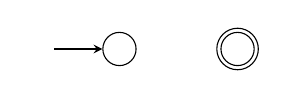
\begin{tikzpicture}[circle]
\node (dummy) at (-1,0) {};
\node (initial) at (0,0) [draw,minimum size=12pt] {};
\node (final) at (1.5,0) [draw,minimum size=15pt] {};
\node at (1.5,0) [draw,minimum size=12pt] {};
\draw[->] (dummy) -- (initial);
\end{tikzpicture}
\end{center}
\item $r$ is the null string $\epsilon$. The NFA consisting of one state which is both initial and final. It accepts the null string:
\begin{center}
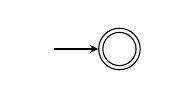
\begin{tikzpicture}[circle]
\node (dummy) at (-1,0) {};
\node (final) at (0,0) [draw,minimum size=15pt] {};
\node at (0,0) [draw,minimum size=12pt] {};
\draw[->] (dummy) -- (final);
\end{tikzpicture}
\end{center}
\item $r$ is a single symbol $a$. The following NFA accepts the language $\{a\}$:
\begin{center}
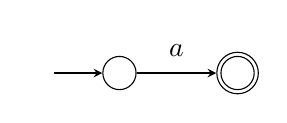
\begin{tikzpicture}[circle]
\node (dummy) at (-1,0) {};
\node (initial) at (0,0) [draw,minimum size=12pt] {};
\node (final) at (1.5,0) [draw,minimum size=15pt] {};
\node at (1.5,0) [draw,minimum size=12pt] {};
\draw[->] (dummy) -- (initial);
\draw[->] (initial) -- node[above] {$a$} (final);
\end{tikzpicture}
\end{center}
\end{itemize}
There are \emph{three} inductive steps:
\begin{itemize}
\item Concatenation $r_1r_2$: By the inductive hypothesis there are NFAs $\mathit{nfa}_1$ and $\mathit{nfa}_2$ that accept the languages of $r_1$ and $r_2$, respectively. Construct $\mathit{nfa}_{12}$ by adding a null transition from the final state of $\mathit{nfa}_1$ to the initial state of $\mathit{nfa}_2$. The initial state of $\mathit{nfa}_{12}$ is the initial state of $\mathit{nfa}_1$ and its final state is the final state of $\mathit{nfa}_2$.
\begin{center}
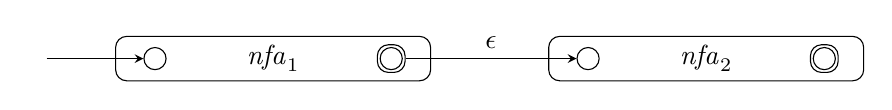
\begin{tikzpicture}[rounded corners]
\node (dummy) at (-3,0) {};
\node at (0,0) [draw,rectangle,minimum width=4cm,minimum height=.5cm] {$\mathit{nfa}_1$};
\node (initial) at (-1.5,0) [draw,minimum size=8] {};
\node (final1) at (1.5,0) [draw,minimum size=10pt] {};
\node at (1.5,0) [draw,minimum size=8] {};
\node at (5.5,0) [draw,rectangle,minimum width=4cm,minimum height=.5cm] {$\mathit{nfa}_2$};
\node (initial2) at (4,0) [draw,minimum size=8] {};
\node at (7,0) [draw,minimum size=10pt] {};
\node at (7,0) [draw,minimum size=8] {};
\draw[->] (dummy) -- (initial);
\draw[->] (final1) -- node[above] {$\epsilon$} (initial2);
\end{tikzpicture}
\end{center}

\item Union $r_1+r_2$: By the inductive hypothesis there are NFAs $\mathit{nfa}_1$ and $\mathit{nfa}_2$ that accept the languages of $r_1$ and $r_2$, respectively. Construct $\mathit{nfa}_{12}$ by adding new start and final states and null transitions.
\begin{center}
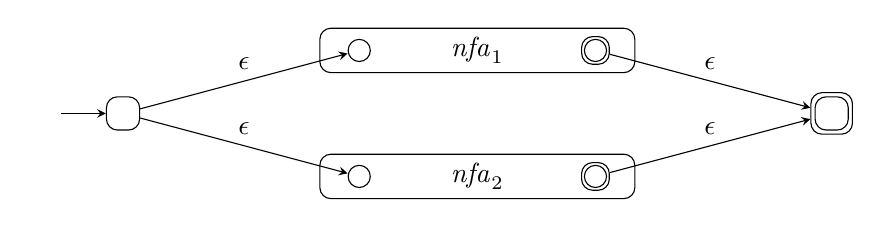
\begin{tikzpicture}[minimum size=12pt,rounded corners]
\node (initial) at (-2,0) [draw] {};
\node (final) at (7,0) [draw,minimum size=15pt] {};
\node at (7,0) [draw] {};
\node (dummy) at (-3,0) {};
\node at (2.5,.8) [draw,rectangle,minimum width=4cm,minimum height=.5cm] {$\mathit{nfa}_1$};
\node at (2.5,-.8) [draw,rectangle,minimum width=4cm,minimum height=.5cm] {$\mathit{nfa}_2$};
\node (top-initial) at (1,.8) [draw,minimum size=8] {};
\node (top-final) at (4,.8) [draw,minimum size=10pt] {};
\node at (4,.8) [draw,minimum size=8] {};
\node (bottom-initial) at (1,-.8) [draw,minimum size=8] {};
\node (bottom-final) at (4,-.8) [draw,minimum size=10pt] {};
\node at (4,-.8) [draw,minimum size=8] {};
\draw[->] (dummy) -- (initial);
\draw[->] (initial) -- node[above] {$\epsilon$} (top-initial);
\draw[->] (initial) -- node[above] {$\epsilon$} (bottom-initial);
\draw[->] (top-final) -- node[above] {$\epsilon$} (final);
\draw[->] (bottom-final) -- node[above] {$\epsilon$} (final);
\end{tikzpicture}
\end{center}

\item Closure $r^*$: By the inductive hypothesis there is an NFA $\mathit{nfa}_r$ that accepts the language of $r$. Add new initial and final states and null transitions as shown in the diagram:
\begin{center}
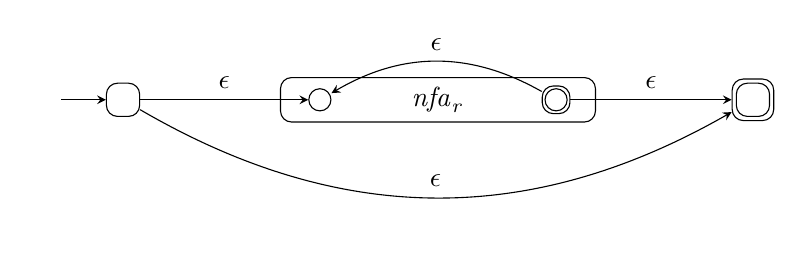
\begin{tikzpicture}[minimum size=12pt,rounded corners]
\node (initial) at (0,0) [draw] {};
\node (final) at (8,0) [draw,minimum size=15pt] {};
\node at (8,0) [draw] {};
\node (initial1) at (2.5,0) [draw,minimum size=8] {};
\node (final1) at (5.5,0) [draw,minimum size=10pt] {};
\node at (5.5,0) [draw,minimum size=8] {};
\draw[->] (final1) to [bend right=30] node[above] {$\epsilon$} (initial1);
\node (dummy) at (-1,0) {};
\node at (4,0) [draw,rectangle,minimum width=4cm,minimum height=.5cm] {$\mathit{nfa}_r$};
\draw[->] (dummy) -- (initial);
\draw[->] (initial) -- node[above] {$\epsilon$} (initial1);
\draw[->] (final1) -- node[above] {$\epsilon$} (final);
\draw[->] (initial) to [bend right=30] node[above] {$\epsilon$} (final);
\end{tikzpicture}
\end{center}
The null transition from the initial state to the final state is taken for strings generated by zero instances of $r$, and the internal transition from the final state of $\mathit{nfa}_r$ to its initial state is for more than one repetition of $r$.
\end{itemize}
\vspace*{-4ex}
\end{proof}

\section{The Well-ordering Principle}\label{s.well}

The well-ordering principle is an axiom that is more intuitive than mathematical induction, although induction is much easier to use in practice.

\begin{definition} Let $S$ be a set with a binary relational operator $\leq$.
\begin{enumerate}
\item $S$ is \emph{totally ordered}\index{Totally ordered} iff for any $x,y\in S$, either $x\leq y$ or $y \leq x$ or $x=y$.
\item A totally ordered set $S$ has a \emph{lower bound}\index{Lower bound} iff there is some $b$ such that $b\leq n$ for all $n\in S$.
\item A totally ordered set $S$ has a \emph{least element}\index{Least element} iff there is some $b\in S$ such that $b\leq n$ for all $n\in S$. A least element is also a lower bound, but in addition it is an element of the set.
\end{enumerate}
\end{definition}
\begin{example}
Subsets of $\mathbb{Z}$ are totally ordered:
\[
S=\{8,3,19,5,6,23\}\,,\quad E_Z=\{\ldots,-4,-2,0,2,4,\ldots\}\,,
\]
where $E_Z$ is the set of all even \emph{integers}. Some lower bounds for $S$ are $3, 0, -10$. The least element of $S$ is $3$. $E_Z$ \emph{does not} have a lower bound and therefore does not have a least element.
\end{example}

\begin{example}
The set of \emph{positive} rational numbers has an infinite number of lower bounds (zero and all negative rational numbers), but it has no least element because for any positive rational number $x$, $x/2$ is a smaller rational number.
\end{example}
\begin{definition} Let $S$ be a totally ordered set. $S$ is \emph{well-ordered} iff \emph{every} nonempty subset of $S$ has a least element.
\end{definition}

$S=\{8,3,19,5,6,23\}$ is well-ordered because every nonempty subset has a least element. The least element of $S$ itself is $3$, the least element of $\{8, 19, 5\}$ is $5$.

$E_Z=\{\ldots,-4,-2,0,2,4,\ldots\}$ is not well-ordered because $E_Z\subseteq E_Z$ but it has no least element. The set of even numbers in $\mathbb{N}$ is well-ordered.

\begin{axiom}\label{ax.wop} \textbf{(The well-ordering principle)}\index{Well-ordering principle} Every nonempty subset of the integers that has a lower bound is well-ordered.
\end{axiom}

The set of positive integers is non-empty and has many lower bounds---zero and all negative integers (and the set even has a least element, namely $1$), therefore by Axiom~\ref{ax.wop} it is well-ordered. If we assume Axiom~\ref{ax.induction} we can prove Axiom~\ref{ax.wop} and conversely [2, 3].


\section{References}

[1] M. Ben-Ari. \textit{Mathematical Logic for Computer Science (Third Edition)}, Springer, 2012, ISBN 978-1-4471-4128-0, \url{http://www.springer.com/978-1-4471-4128-0}.

[2] M. Ben-Ari. \textit{The Many Guises of Induction}, 2019, \url{https://www.weizmann.ac.il/sci-tea/benari/mathematics#induction}.

[3] D.S. Gunderson. \textit{Handbook of Mathematical Induction: Theory and Applications}, Mathematical Association of America, 2010.

[4] D.J. Velleman. \textit{How to Prove It: A Structured Approach (Second Edition)}, Cambridge University Press, 2006.

\balance
\printindex
\end{document}
